%%
%% This is file `tikzposter-template.tex',
%% generated with the docstrip utility.
%%
%% The original source files were:
%%
%% tikzposter.dtx  (with options: `tikzposter-template.tex')
%%
%% This is a generated file.
%%
%% Copyright (C) 2014 by Pascal Richter, Elena Botoeva, Richard Barnard, and Dirk Surmann
%%
%% This file may be distributed and/or modified under the
%% conditions of the LaTeX Project Public License, either
%% version 2.0 of this license or (at your option) any later
%% version. The latest version of this license is in:
%%
%% http://www.latex-project.org/lppl.txt
%%
%% and version 2.0 or later is part of all distributions of
%% LaTeX version 2013/12/01 or later.
%%


\documentclass{tikzposter} %Options for format can be included here

\usepackage{todonotes}

\usepackage[tikz]{bclogo}
\usepackage{lipsum}
\usepackage{amsmath}

\usepackage{booktabs}
\usepackage{longtable}
\usepackage[absolute]{textpos}
\usepackage[it]{subfigure}
\usepackage{graphicx}
\usepackage{cmbright}
%\usepackage[default]{cantarell}
%\usepackage{avant}
%\usepackage[math]{iwona}
\usepackage[math]{kurier}
\usepackage[T1]{fontenc}


%% add your packages here
\usepackage{hyperref}
% for random text
\usepackage{lipsum}
\usepackage[english]{babel}
\usepackage[pangram]{blindtext}

\colorlet{backgroundcolor}{blue!10}

 % Title, Author, Institute
\title{Group Outlying Aspects Mining}
\author{Jincai Ma}
\institute{ Xi'an Shiyou University, China \\
}
%\titlegraphic{logos/tulip-logo.eps}

%Choose Layout
\usetheme{Wave}

%\definebackgroundstyle{samplebackgroundstyle}{
%\draw[inner sep=0pt, line width=0pt, color=red, fill=backgroundcolor!30!black]
%(bottomleft) rectangle (topright);
%}
%
%\colorlet{backgroundcolor}{blue!10}

\begin{document}


\colorlet{blocktitlebgcolor}{blue!23}

 % Title block with title, author, logo, etc.
\maketitle

\begin{columns}
 % FIRST column
\column{0.5}% Width set relative to text width

%%%%%%%%%% -------------------------------------------------------------------- %%%%%%%%%%
 %\block{Main Objectives}{
%  	      	\begin{enumerate}
%  	      	\item Formalise research problem by extending \emph{outlying aspects mining}
%  	      	\item Proposed \emph{GOAM} algorithm is to solve research problem
%  	      	\item Utilise pruning strategies to reduce time complexity
%  	      	\end{enumerate}
%%  	      \end{minipage}
%}
%%%%%%%%%% -------------------------------------------------------------------- %%%%%%%%%%


%%%%%%%%%% -------------------------------------------------------------------- %%%%%%%%%%
\block{Introduction}{
  
  	
    \begin{description}
    \item [Project Background]  Bike-sharing is not new to us. This report mainly analyzes the data of bike-sharing in Washington, US from 2011 to 2012.
      
  	\item[The Data Source] The data comes from Kaggle https://www.kaggle.com/c/bike-sharing-demand
  	
  	\item[Project Purpose] This project is mainly about the prediction of relevant data, and the description and analysis of relevant factors are presented here.
  	\end{description}

  	
}
%%%%%%%%%% -------------------------------------------------------------------- %%%%%%%%%%


%%%%%%%%%% -------------------------------------------------------------------- %%%%%%%%%%
\block{Related Field Name Interpretation}{

\begin{itemize}
    \item
    datetime
    season 
    holiday 
    workingday 
    weather
    temp \\  atemp 
    humidity 
    windspeed 
    casual 
    registered 
    count 
\end{itemize}


}
%%%%%%%%%% -------------------------------------------------------------------- %%%%%%%%%%


%%%%%%%%%% -------------------------------------------------------------------- %%%%%%%%%%

%\note{Note with default behavior}

%\note[targetoffsetx=12cm, targetoffsety=-1cm, angle=20, rotate=25]
%{Note \\ offset and rotated}

 % First column - second block


%%%%%%%%%% -------------------------------------------------------------------- %%%%%%%%%%
\block{ Data Analysis}{
                                       
    \begin{itemize}
        \item
        Descriptive statistics of the data
    \end{itemize}
    \begin{minipage}{1\linewidth}
        \centering
        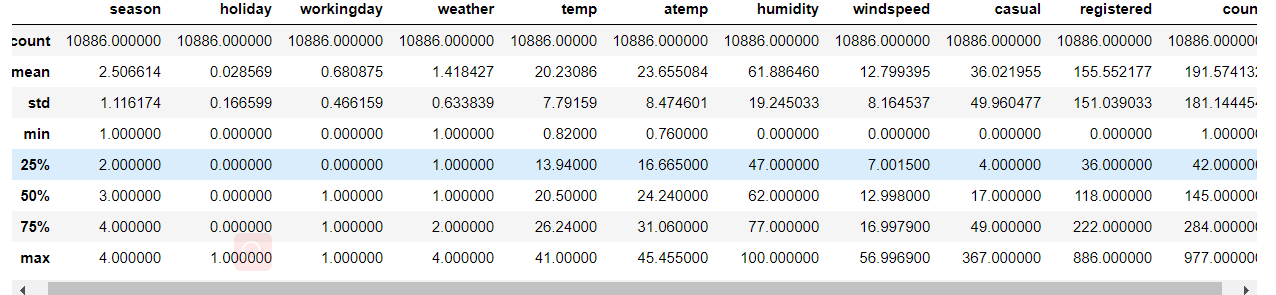
\includegraphics[width=1\textwidth]{pic1/a.png} 
    \end{minipage}

  
    \begin{itemize}   
        \item
        The standard deviation of the number of leases you have to predict at the end is very large.So let's look at the distribution by drawing it.                         
        \item
        Exclude data other than three standards,log of count
    \end{itemize}
    \begin{minipage}{0.3\linewidth}
        \centering
        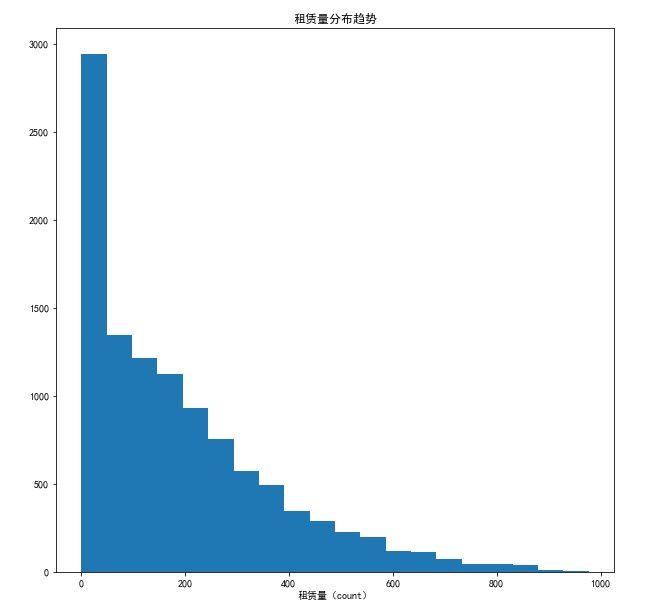
\includegraphics[width=0.7\textwidth]{pic1/count.png} 
    \end{minipage}
    \begin{minipage}{0.33\linewidth}
        \centering
        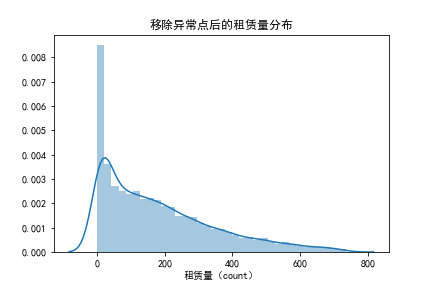
\includegraphics[width=1\textwidth]{pic1/count2.png} 
    \end{minipage}
    \begin{minipage}{0.33\linewidth}
        \centering
        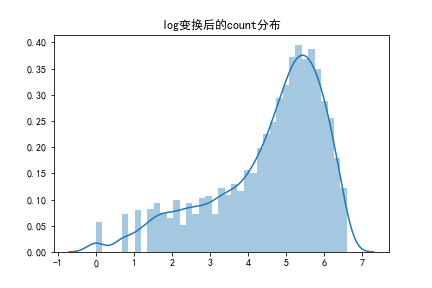
\includegraphics[width=1\textwidth]{pic1/log.png} 
    \end{minipage}
    \begin{itemize}                            
        \item
        The impact of hour,month,season,year,weekday,workingday
    \end{itemize}
    \begin{minipage}{1\linewidth}
        \centering
        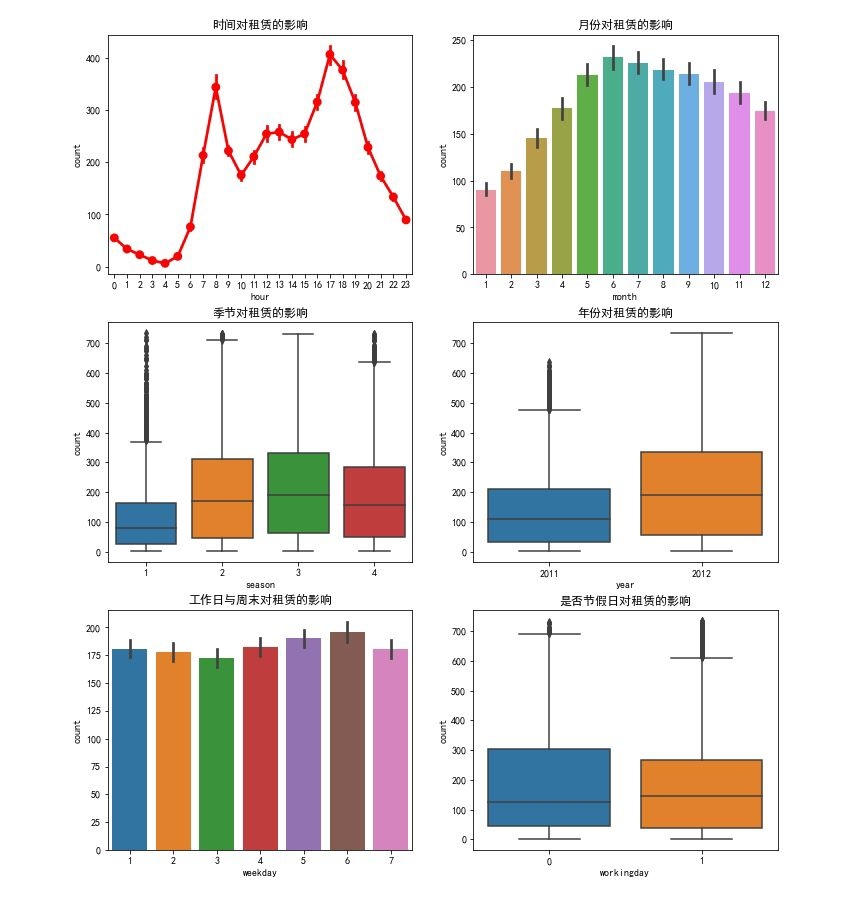
\includegraphics[width=0.5\textwidth]{pic1/count all.png} 
    \end{minipage}
    \begin{itemize}                            
        \item
        The impact of weather
    \end{itemize}
    \begin{minipage}{1\linewidth}
        \centering
        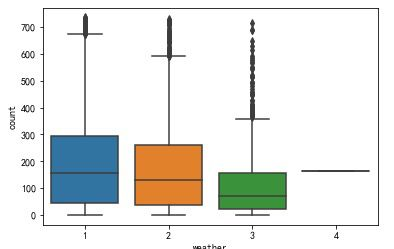
\includegraphics[width=0.4\textwidth]{pic1/weather.png} 
    \end{minipage}
}
%%%%%%%%%% -------------------------------------------------------------------- %%%%%%%%%%


% SECOND column
\column{0.5}
 %Second column with first block's top edge aligned with with previous column's top.

%%%%%%%%%% -------------------------------------------------------------------- %%%%%%%%%%
\block{Data Analysis}{
    
    \begin{itemize}                            
        \item
        The impact of temp,atemp,humidity,windspeed
    \end{itemize}
    \begin{minipage}{0.5\linewidth}
        \centering
        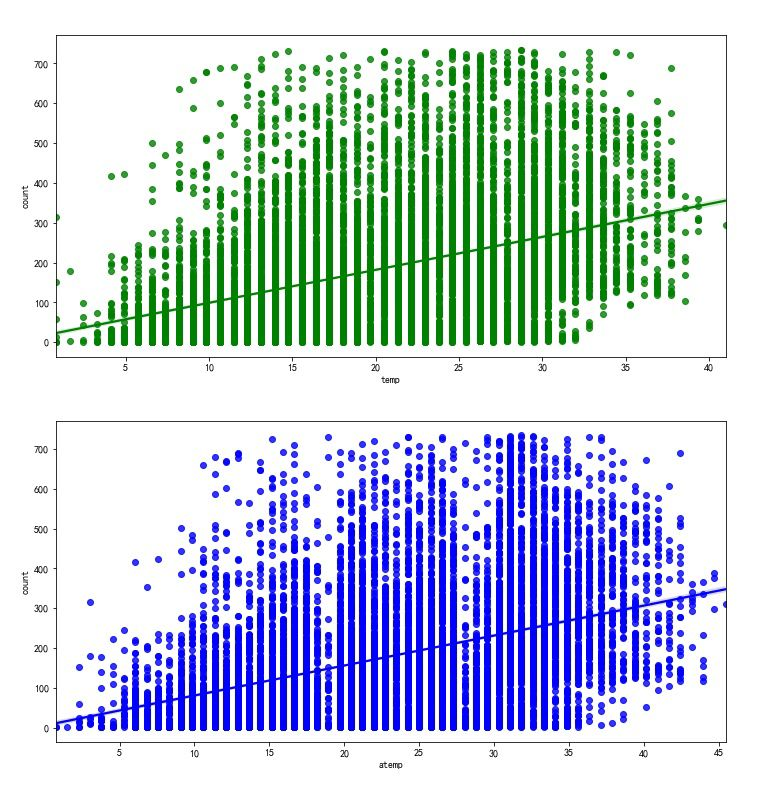
\includegraphics[width=0.7\textwidth]{pic1/three tahw1 (1).png} 
    \end{minipage}
    \begin{minipage}{0.4\linewidth}
        \centering
        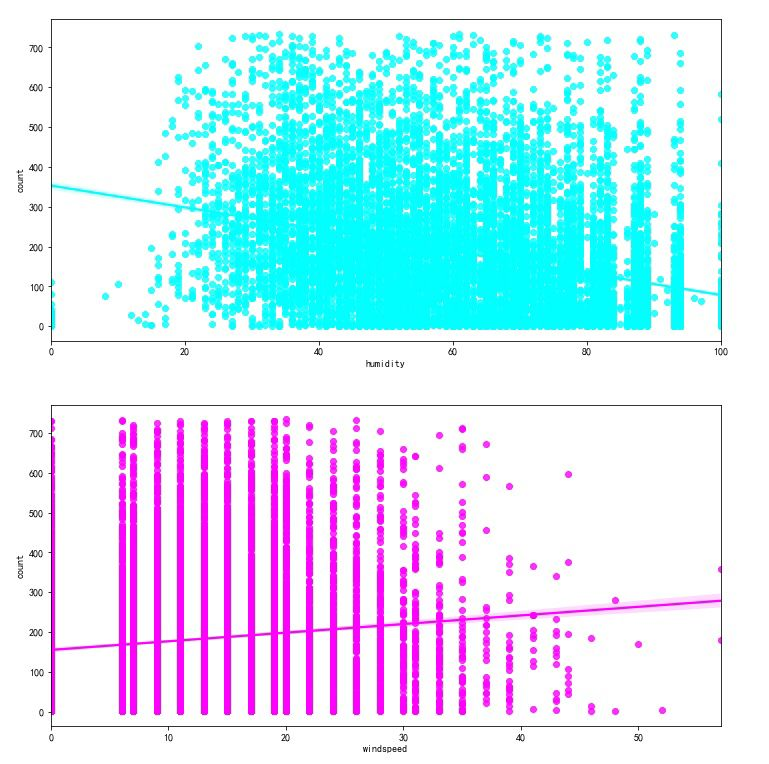
\includegraphics[width=0.7\textwidth]{pic1/three tahw2.png} 
    \end{minipage}
   
}
%%%%%%%%%% -------------------------------------------------------------------- %%%%%%%%%%
% Second column - first block
\block{Data Analysis}{
   
    \begin{itemize}                            
        \item
        Impact of season,week,registered and non-registered users on cycling usage trends
    \end{itemize}
    \begin{minipage}{0.33\linewidth}
        \centering
        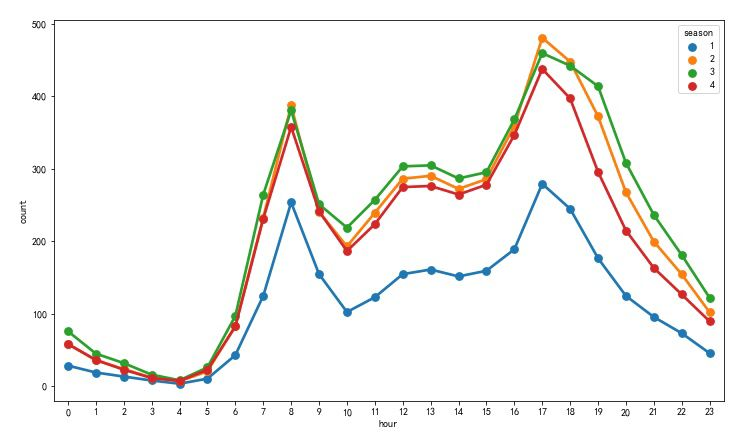
\includegraphics[width=1\textwidth]{pic1/three hour1.png} 
    \end{minipage}
    \begin{minipage}{0.33\linewidth}
        \centering
        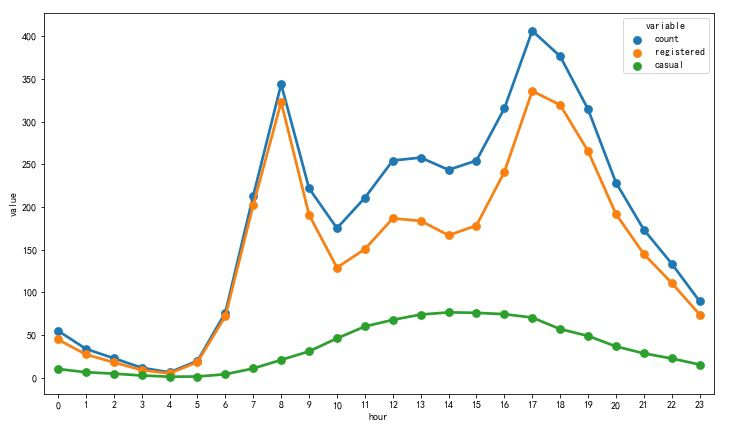
\includegraphics[width=1\textwidth]{pic1/three hour3.png} 
    \end{minipage}
    \begin{minipage}{0.33\linewidth}
        \centering
        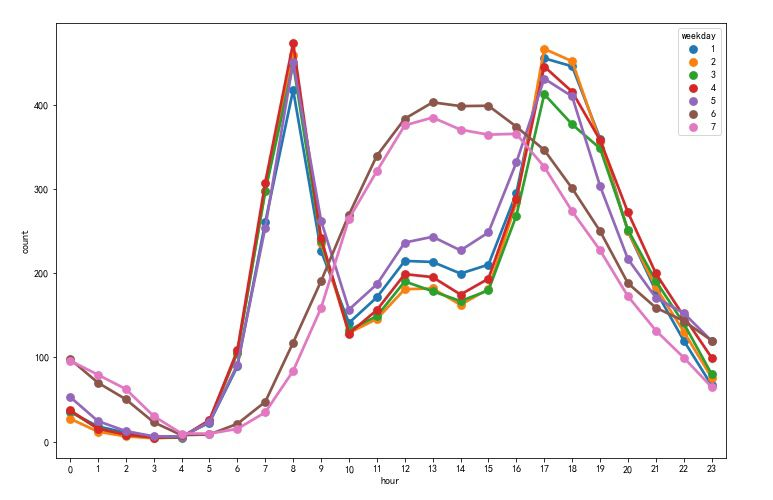
\includegraphics[width=1\textwidth]{pic1/three hour2.png} 
    \end{minipage}

    \begin{itemize}                            
        \item
        Draw the thermal diagram of the correlation coefficient
    \end{itemize}
    \begin{minipage}{1\linewidth}
        \centering
        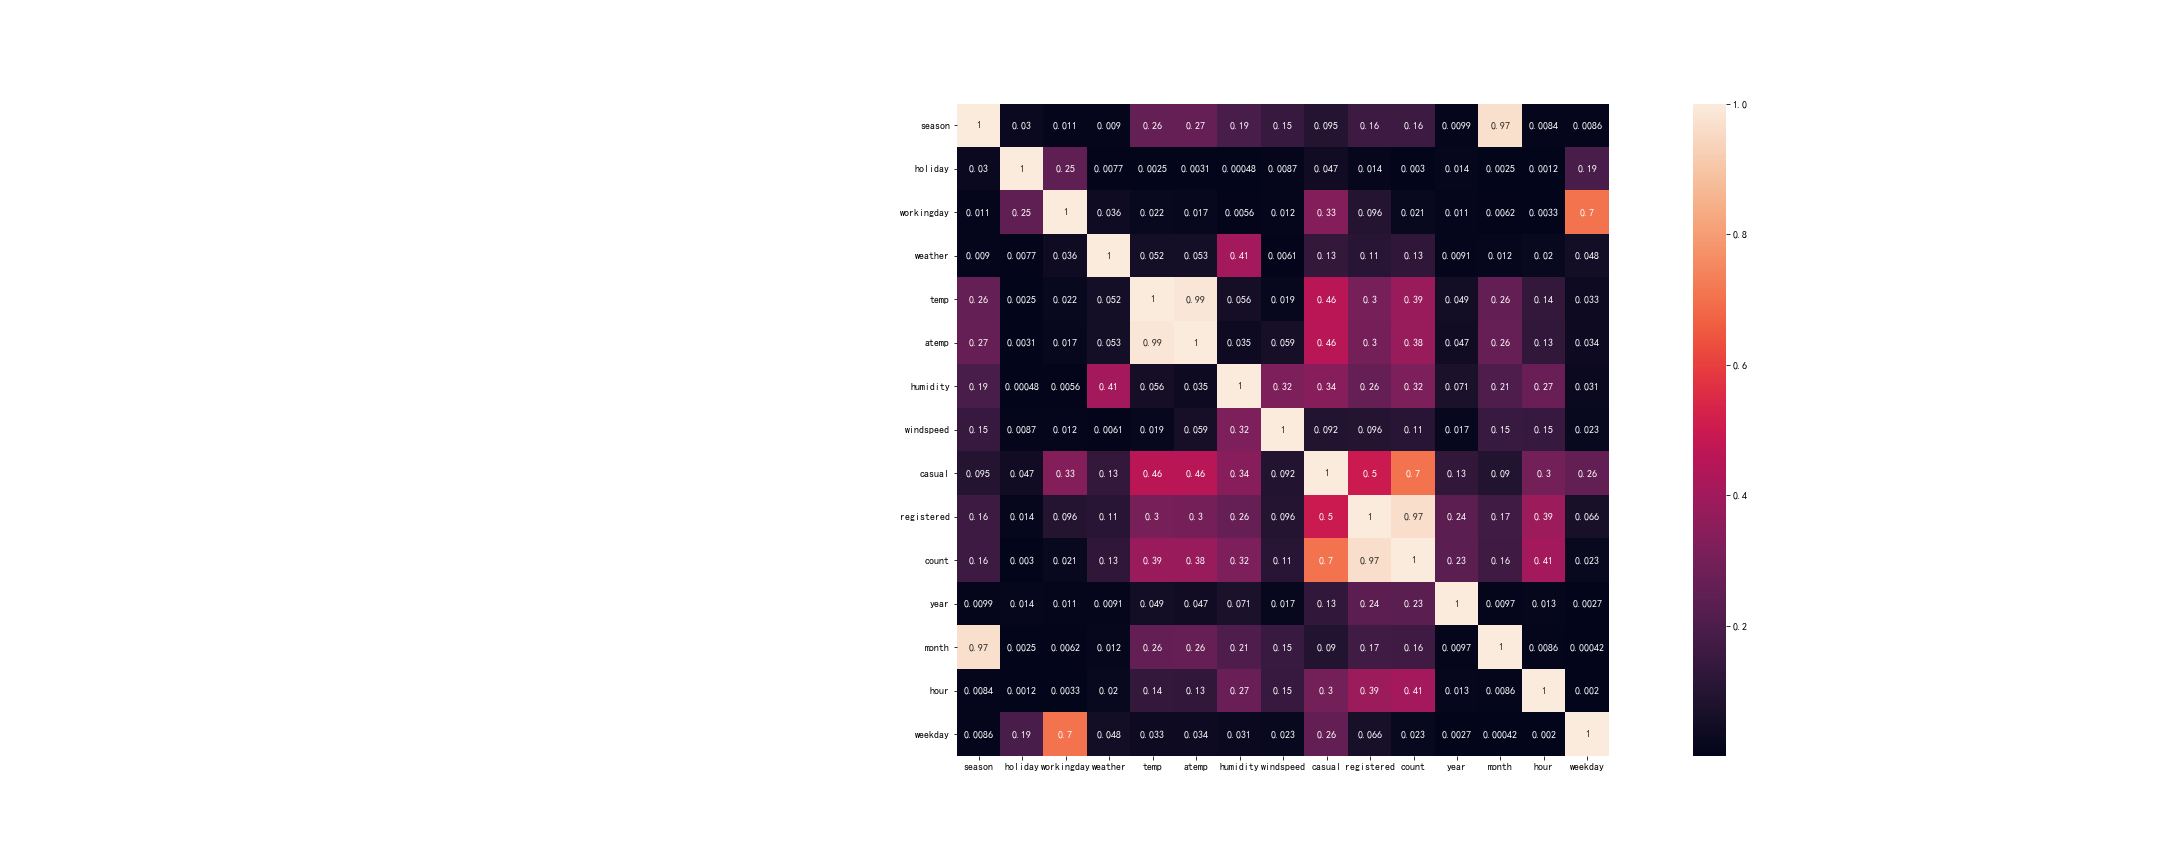
\includegraphics[width=0.6\textwidth]{pic1/hot.png} 
    \end{minipage}
    It can be seen that the correlation from large to small is:registered    casual  hour  temp   atemp  year   month  season  windspeed     weekday       holiday workingday   weather      
    humidity     
}

%%%%%%%%%% -------------------------------------------------------------------- %%%%%%%%%%
\block{Build Model}{

\begin{description}
    \item[]
    1.Separate the training set and test set.\\
    2.Remove unwanted eigenvalues:'casual','count','datetime','registered','date','atemp','month','year','season','weather'\\
    3.Cross validation is used to determine the optimal parameters.\\
    4.View the selected optimal parameters:{max depth: 20, n estimators: 150}\\
    5.Apply the optimal parameters to the model, it can be obtained\\
    Accuracy on test set : 0.6945996275605214
\end{description}


}
%%%%%%%%%% -------------------------------------------------------------------- %%%%%%%%%%


% Second column - second block
%%%%%%%%%% -------------------------------------------------------------------- %%%%%%%%%%
\block[titlewidthscale=1, bodywidthscale=1]
{Conclusion}
{
\begin{description}
  \item[]
  Through this Kaggle project, I practiced by myself to have a deeper understanding of data visualization and to explore the structure and rules of data by means of drawing and tabulating.

\end{description}
}
%%%%%%%%%% -------------------------------------------------------------------- %%%%%%%%%%


% Bottomblock
%%%%%%%%%% -------------------------------------------------------------------- %%%%%%%%%%
\colorlet{notebgcolor}{blue!20}
\colorlet{notefrcolor}{blue!20}
\note[targetoffsetx=8cm, targetoffsety=-4cm, angle=30, rotate=15,
radius=2cm, width=.26\textwidth]{
Acknowledgement
\begin{itemize}
    \item
    International Cooperation Project (Y7Z0511101)
    of IIE,
    Chinese Academy of Sciences
 \end{itemize}
}

%\note[targetoffsetx=8cm, targetoffsety=-10cm,rotate=0,angle=180,radius=8cm,width=.46\textwidth,innersep=.1cm]{
%Acknowledgement
%}

%\block[titlewidthscale=0.9, bodywidthscale=0.9]
%{Acknowledgement}{
%}
%%%%%%%%%% -------------------------------------------------------------------- %%%%%%%%%%

\end{columns}


%%%%%%%%%% -------------------------------------------------------------------- %%%%%%%%%%
%[titleleft, titleoffsetx=2em, titleoffsety=1em, bodyoffsetx=2em,%
%roundedcorners=10, linewidth=0mm, titlewidthscale=0.7,%
%bodywidthscale=0.9, titlecenter]

%\colorlet{noteframecolor}{blue!20}
\colorlet{notebgcolor}{blue!20}
\colorlet{notefrcolor}{blue!20}
\note[targetoffsetx=-13cm, targetoffsety=-13cm,rotate=0,angle=180,radius=8cm,width=.96\textwidth,innersep=.4cm]
{
\begin{minipage}{0.3\linewidth}
\centering

\includegraphics[width=24cm]{logos/tulip-wordmark.eps}
\end{minipage}
\begin{minipage}{0.7\linewidth}
{ \centering
 The $11^{th}$ International Conference on Knowledge Science,
  Engineering and Management (KSEM 2018),
  17-16/20/2020,Xi'an, China
}
\end{minipage}
}
%%%%%%%%%% -------------------------------------------------------------------- %%%%%%%%%%


\end{document}

%\endinput
%%
%% End of file `tikzposter-template.tex'.
